\section{Optymalizacja kombinatoryczna}

%%%%%%%%%%%%%%%% 
	\begin{frame}{Optymalizacja kombinatoryczna }
		\begin{exampleblock}{Problem komiwojażera}
			\begin{itemize}
				\item \textbf{In}: symetryczna macierz odległości $(N*N)$
						
				\item \textbf{Out}: permutacja zbioru $\{1,2,...,N\}$ taka, że np:
					$$
						L_{min} = \sum_{i=1}^N \{ \underbrace{(|x_i - x_{i+1}| + |y_i - y_{i+1}|)}_\text{odległość w metryce Manhattan} + \underbrace{\lambda(\mu_i - \mu_{i-1})}_\text{funkcja kary (penalty)}\}
					$$
			\end{itemize}		
			%DEAD LINK
			%Demo optymalizacji problemu komiwojażera (autor: Maciej Borowiec): \url{komiwojazer/komiwojazer.html} 
		\end{exampleblock}
		
	\end{frame}
%%%%%%%%%%%%%%%%

	\begin{frame}{Optymalizacja kombinatoryczna}
		\begin{exampleblock}{Zagadnienia NP-zupełne (nondeterministic polynomial)}
			\begin{itemize}
				\item rozwiązania o złożoności $\sim e^N$
				\item wiele stopni swobody
				\item dyskretne (wykluczone poszukiwanie w kierunku)
				\item funkcja celu (L) łączy przeciwstawne cele cząstkowe			
			\end{itemize}
		\end{exampleblock}
		Dobry przegląd w \cite{garey}
	\end{frame}
	
%%%%%%%%%%%%%%%%
\subsection{Typowa funkcja celu}
	\begin{frame}{Typowa funkcja celu}
		\begin{itemize}
			\item skalar: wsystkie cele sprowadza do jednego
			\item wiele lokalnych minimów - rzędu $e^N$
			\item w praktyce - potrzebne dobre rozwiązanie - nie musi być to minimum globalne	
		\end{itemize}

	\end{frame}

%%%%%%%%%%%%%%%%

	\begin{frame}{Typowa funkcja celu}
		\begin{figure}
			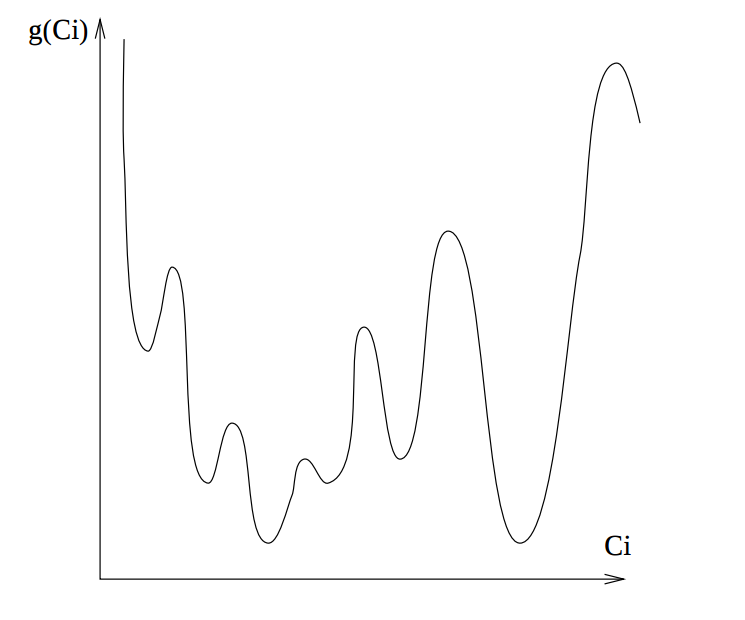
\includegraphics[height=0.9\textheight]{img/18/target_fun}
		\end{figure}
	\end{frame}	
	
%%%%%%%%%%%%%%%%

	\begin{frame}{Typowa funkcja celu}
		Niezbędne:
		\begin{itemize}
			\item $C_i$ - reprezentacja konfiguracji układu
			\item $g(C_i)$
			\item procedura generacji kolejnych konfiguracji
		\end{itemize}
	\end{frame}	
	
%%%%%%%%%%%%%%%%	
	
	\begin{frame}{Przykład procedury generacji nowych konfiguracji}
		\begin{exampleblock}{TSP \cite{lin}}
			Heurystyka: \textit{iterative improvement} - akceptowalne zmiany zmniejszające funkcję celu
			\begin{enumerate}
				\item odwrócenie kolejności obiegu 5-ciu górnych
				\item wstawienie 5-ciu górnych między 2 dolne
			\end{enumerate}	
			$\rightarrow$ pewne ugrzęźnięcie w lokalnym minimum			
			\begin{figure}
				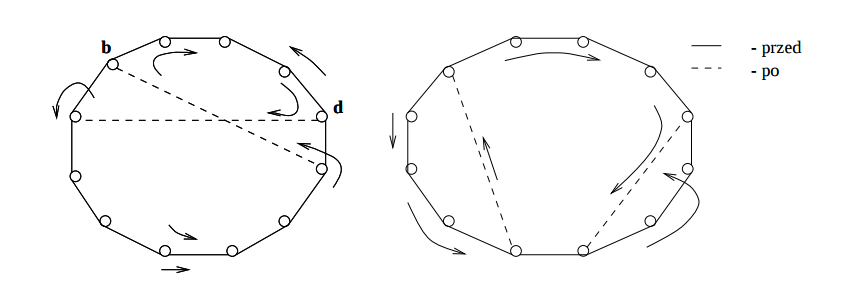
\includegraphics[height=0.4\textheight]{img/18/tsp}
			\end{figure}
		\end{exampleblock}
	\end{frame}
	

